\documentclass[]{article}
\usepackage{lmodern}
\usepackage{amssymb,amsmath}
\usepackage{ifxetex,ifluatex}
\usepackage{fixltx2e} % provides \textsubscript
\ifnum 0\ifxetex 1\fi\ifluatex 1\fi=0 % if pdftex
  \usepackage[T1]{fontenc}
  \usepackage[utf8]{inputenc}
\else % if luatex or xelatex
  \ifxetex
    \usepackage{mathspec}
    \usepackage{xltxtra,xunicode}
  \else
    \usepackage{fontspec}
  \fi
  \defaultfontfeatures{Mapping=tex-text,Scale=MatchLowercase}
  \newcommand{\euro}{€}
\fi
% use upquote if available, for straight quotes in verbatim environments
\IfFileExists{upquote.sty}{\usepackage{upquote}}{}
% use microtype if available
\IfFileExists{microtype.sty}{%
\usepackage{microtype}
\UseMicrotypeSet[protrusion]{basicmath} % disable protrusion for tt fonts
}{}
\usepackage[margin=1in]{geometry}
\usepackage{graphicx}
\makeatletter
\def\maxwidth{\ifdim\Gin@nat@width>\linewidth\linewidth\else\Gin@nat@width\fi}
\def\maxheight{\ifdim\Gin@nat@height>\textheight\textheight\else\Gin@nat@height\fi}
\makeatother
% Scale images if necessary, so that they will not overflow the page
% margins by default, and it is still possible to overwrite the defaults
% using explicit options in \includegraphics[width, height, ...]{}
\setkeys{Gin}{width=\maxwidth,height=\maxheight,keepaspectratio}
\ifxetex
  \usepackage[setpagesize=false, % page size defined by xetex
              unicode=false, % unicode breaks when used with xetex
              xetex]{hyperref}
\else
  \usepackage[unicode=true]{hyperref}
\fi
\hypersetup{breaklinks=true,
            bookmarks=true,
            pdfauthor={Ren Zhang},
            pdftitle={Test a Perceptual Phenomenon},
            colorlinks=true,
            citecolor=blue,
            urlcolor=blue,
            linkcolor=magenta,
            pdfborder={0 0 0}}
\urlstyle{same}  % don't use monospace font for urls
\setlength{\parindent}{0pt}
\setlength{\parskip}{6pt plus 2pt minus 1pt}
\setlength{\emergencystretch}{3em}  % prevent overfull lines
\setcounter{secnumdepth}{5}

%%% Use protect on footnotes to avoid problems with footnotes in titles
\let\rmarkdownfootnote\footnote%
\def\footnote{\protect\rmarkdownfootnote}

%%% Change title format to be more compact
\usepackage{titling}

% Create subtitle command for use in maketitle
\newcommand{\subtitle}[1]{
  \posttitle{
    \begin{center}\large#1\end{center}
    }
}

\setlength{\droptitle}{-2em}
  \title{Test a Perceptual Phenomenon}
  \pretitle{\vspace{\droptitle}\centering\huge}
  \posttitle{\par}
  \author{Ren Zhang}
  \preauthor{\centering\large\emph}
  \postauthor{\par}
  \predate{\centering\large\emph}
  \postdate{\par}
  \date{September 27, 2015}



\begin{document}

\maketitle


{
\hypersetup{linkcolor=black}
\setcounter{tocdepth}{2}
\tableofcontents
}
\subsection{Introduction}\label{introduction}

In this paper, we are analyzing a sample test results from the Stroop
effect experiment. The participants in the experiment are required to
name the color of the ink of a list of words shown on screen in two
different settings. In one setting, the words that are congruent with
the color of ink, and in the other setting the words that are
incongruent with their color of ink. The time it takes to finish each
test are recorded for further analysis

\subsection{Variables of Interest}\label{variables-of-interest}

\begin{itemize}
\itemsep1pt\parskip0pt\parsep0pt
\item
  The independent variable is the type of test, which could be congruent
  or incongruent.\\
\item
  The dependent variable is the time it takes for participants to
  complete the task.
\end{itemize}

\subsection{Hypothesis}\label{hypothesis}

\begin{itemize}
\itemsep1pt\parskip0pt\parsep0pt
\item
  The null hypotheses is: The average time it takes to complete the
  incongruent test is less than or equal to the average time needed to
  complete the congruent test.\\
\item
  The alternative hypotheses is: The average time it takes to complete
  the incongruent test is more than the average time needed to complete
  the congruent test.\\
\item
  The appropriate test is a paired sampe right-tailed t-test, we use
  this test because the data is a matched pairs sample, and the
  inference we want to make is that the parameter is greater than the
  hypothesized value.
\end{itemize}

\subsection{Descriptive Statistics}\label{descriptive-statistics}

\begin{itemize}
\itemsep1pt\parskip0pt\parsep0pt
\item
  For the congruent setting test, the average finishing time is
  14.051125, and the corrected standard deviation is 3.559358.\\
\item
  For the incongruent setting test, the average finishing time is
  22.0159167 and the corrected standard deviation is 4.7970571.\\
\item
  The sample mean of the time difference is 7.9647917, and the standard
  deviation is 4.8648269.
\end{itemize}

\subsection{Visualizations}\label{visualizations}

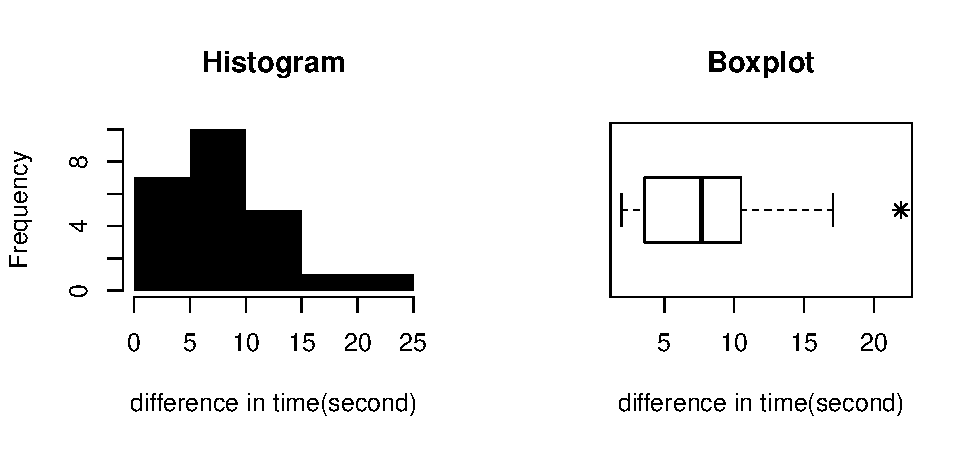
\includegraphics{draft_files/figure-latex/unnamed-chunk-3-1.pdf} The
distribution is positivly skwed, and their is one observation we might
want to classify as an outlier.

\subsection{Statistical Test}\label{statistical-test}

The confidence level used here is the default 95\% level, the test
statistic calculated here is 8.0207069, the critical value is 1.7138715,
since the test statistic is greater than the critical value, we reject
the null hypothesis and conclude that the average time it takes a person
to complete the test in an incongruent setting is longer than the time
it takes for the same person to complete a congruent setting test.

An output from statistical software for this test is included in the
Appendix.

\subsection{Further Thoughts}\label{further-thoughts}

We might conduct studies to see whether smell would interference the
visual perception. We may place papers with words describing different
smells on them and placed them under transparent containers, wherein
each container we put things with a strong smell that is different from
the word printed on the paper. In another setting we match the things we
put in the container with the descriptive words underneath the
container. And we can conduct a similar test to the Stroop test to see
how it turn out.

\pagebreak  

\subsection{Appendix: R output for the
t-test}\label{appendix-r-output-for-the-t-test}

\begin{verbatim}
## 
##  Paired t-test
## 
## data:  data$Incongruent and data$Congruent
## t = 8.0207, df = 23, p-value = 2.052e-08
## alternative hypothesis: true difference in means is greater than 0
## 95 percent confidence interval:
##  6.262868      Inf
## sample estimates:
## mean of the differences 
##                7.964792
\end{verbatim}

\end{document}
